\documentclass[11pt, onecolumn]{article}
\usepackage{hyperref}
\usepackage{url}
%\usepackage{mathpazo,mathrsfs}
%\usepackage[T1]{fontenc}

%\usepackage[usenames,dvipsnames]{color}
\usepackage{stmaryrd} \usepackage{url} \usepackage[latin1]{inputenc}
\usepackage{graphicx}% Include figure files
\usepackage{amssymb} \usepackage{subfigure} \usepackage{amsmath}
\usepackage{amsthm}
\usepackage{dcolumn}% Align table columns on decimal point
\usepackage{bm}% bold math
\usepackage{color}
\usepackage{mathtools}


%\usepackage{algorithm} \usepackage{algorithmic}
\usepackage[noline,boxed]{algorithm2e}

\newcommand{\alert}[1]{\textcolor{red}{#1}} \newcommand{\vect}[1]{\boldsymbol{#1}}
\newcommand{\todo}[1]{\vspace{5 mm}\par \noindent \framebox{\begin{minipage}[c]{8cm} \tt
      #1
    \end{minipage}}\vspace{5 mm}\par}

\newcommand{\STATE}{\quad}
\newcommand{\COMMENT}[1]{{\sl (#1)}}
\newcommand{\RETURN}{\tb{Return }}

\newtheorem{theorem}{Theorem}[section]
\newtheorem{statement}[theorem]{Statement}
\newtheorem{proposition}[theorem]{Proposition}
\newtheorem{lemma}[theorem]{Lemma}
\newtheorem{corollary}[theorem]{Corollary}
\newtheorem{question}[theorem]{Question}
\newtheorem{remark}[theorem]{Remark}
\newtheorem{conjecture}{Conjecture}
\newtheorem{claim}[theorem]{Claim}
\newtheorem{condition}[theorem]{Condition}
\newtheorem*{subproblem*}{Subproblem}
\newtheorem{definition}[theorem]{Definition} \newtheorem{example}{Example}
\newtheorem{assumption}{Assumption} \newtheorem{scenario}{Scenario}
\newtheorem{step}{Step} \newtheorem{steps}{Step} \newtheorem{stp}{Step}
\newtheorem{stps}{Step} \newtheorem{problem}{Problem}

%\newenvironment{proof}[1][Proof]{\begin{trivlist}
%\item[\hskip \labelsep {\bfseries #1}]}{\end{trivlist}}


\usepackage{hyperref}

%\renewcommand{\algorithmicrequire}{\textbf{Input:}}
%\renewcommand{\algorithmicensure}{\textbf{Output:}}
%\renewcommand{\algorithmireturn}{\textbf{Return:}}



%\usepackage[dvips]{graphicx}
% \usepackage{amsfonts,mathrsfs,amsfonts, array, geometry}
% \usepackage{graphicx,amsmath,amssymb,multirow} \setcounter{MaxMatrixCols}{30}%
% \usepackage[usenames]{color} \usepackage[usenames, dvipsnames]{xcolor}
% \usepackage{epstopdf}\usepackage{framed}
% \usepackage{algpseudocode}
% \usepackage{ulem}

% \newtheorem{Thm}{Theorem} \newtheorem{Lem}{Lemma} \newtheorem{Cor}{Corollary}
% \newtheorem{Def}{Definition} \newtheorem{Exam}{Example} \newtheorem{Alg}{Algorithm}
% \newtheorem{Prob}{Problem} \newtheorem{Rem}{Remark} \newtheorem{Proof}{Proof}
% \newtheorem{Prop}{Proposition} \newtheorem{Assump}{Assumption}

\newcommand{\mc}{\mathcal}
\newcommand{\mb}{\mathbf} \newcommand{\mbb}{\mathbb} \newcommand{\wt}{\widetilde}
\newcommand{\fa}{\forall} \newcommand{\tc}{\textcolor} \newcommand{\tb}{\textbf}
\newcommand{\tx}{\text} \newcommand{\tcws}{\textcolor{WildStrawberry}}
\newcommand{\tcbl}{\textclor{blue}}
\newcommand{\p}{\partial}
\newcommand{\dr}{\text{d}}
\newcommand{\bs}{\boldsymbol}
\newcommand{\ot}{\otimes}

\newcommand{\ta}{\theta}
\newcommand{\Ta}{\Theta}

\newcommand{\Proj}{\mbox{Proj}}
\newcommand{\R}{\mbb R}
\newcommand{\C}{\mbb C}
\newcommand{\Z}{\mbb Z}
\newcommand{\E}{\mbb E}

\newcommand{\ul}{\underline}
\newcommand{\ol}{\overline}
\newcommand{\wh}{\widehat}
\newcommand{\prj}{\tx{Proj}}
% \newcommand{\mog}{Gaussian mixture model}
\newcommand{\mog}{mixture of Gaussians }
% \newcommand{\mog}{MoG}
\newcommand{\vc}{\tx{vec}}
\newcommand{\mt}{\tx{mat}}
\newcommand{\diag}{\tx{diag}}
\newcommand{\poly}{\tx{poly}}
\newcommand{\cond}{\tx{cond}}
\newcommand{\ep}{\tx{exp}}
\newcommand{\lt}{\left}
\newcommand{\rt}{\right}

\newcommand{\defeq}{\vcentcolon=}
\newcommand{\eqdef}{=\vcentcolon}
\newcommand{\od}{\odot}

%\linespread{1}
%\let\labelindent\relax
\usepackage{enumitem}
\usepackage[margin=1in]{geometry}

\newcommand{\qq}[1]{{\color{magenta}{(#1)}}}
\newcommand{\rb}[1]{{\color{red}{ #1}}}
\newcommand{\bl}[1]{{\color{blue}{ #1}}}
\iffalse
\fi

{
 \theoremstyle{plain}
      \newtheorem{asm}{Assumption}
}
\theoremstyle{plain}
\newtheorem{thm}{Theorem}[section]
%\newtheorem{claim}[thm]{Claim}
\newtheorem{lem}[thm]{Lemma}
\newtheorem{cor}[thm]{Corollary}


\newtheorem{prop}[thm]{Proposition}

\theoremstyle{definition}
\newtheorem{defn}{Definition}[section]
\newtheorem{conj}{Conjecture}[section]
\newtheorem{exmp}{Example}[section]
\newtheorem{exc}{Exercise}[section]


\begin{document}
\title{controller validation for uncertain systems}
\date{\today}

%\maketitle
%\thispagestyle{empty}
%\pagestyle{empty}

% \begin{abstract}
% \end{abstract}
% \begin{keywords}
% \end{keywords}

\setcounter{page}{1}


\section{ID-Control Problem}
%The goal is to use IQC constraints to replace the clear-cut between sys id and controller synthesis.

We have open loop / closed loop experiment data (which gives information about the unknown plant $P$), a
candidate controller $K$, and a set of closed-loop performance specification $T_{spec}$.

The control question is whether the closed loop system of the controller $K$ and the unknown plant
$P$ will meet the performance specification $T_{spec}$.
%
To answer that, we need an algorithm to directly check the consistency among data, controller, and
$T_{spec}$.
%
The sample complexity is to quantify how much we need to know from data in order to confidently
answer the question.
%
The ultimate goal of controller invalidation is that we want to efficiently prune the suboptimal
controllers to select the one that achieves optimal closed loop performance.

\paragraph{To do list }
\begin{enumerate}
\item Pin down the details of the algorithm for controller invalidation using S-proc.
\item Bound sample complexity of controller invalidation, under the assumptions about true plant and noise
  model.
\item Better experiment design for 1. open loop experiment and 2. how to prune the set of candidate controllers.
\item Simulation of the simple setting to see how it works (with IQC synthesis)
\end{enumerate}

\subsection{Algorithm for Controller Invalidation}

\paragraph{Step 1,  collect open loop experiment data}
Run open loop experiment for unknown plant $P$ to obtain $N$ pairs of length-$T$ signals $\{(s_i,v_i) :
i=1,\dots, N\}$.
\begin{figure}[!ht]
  \centering
  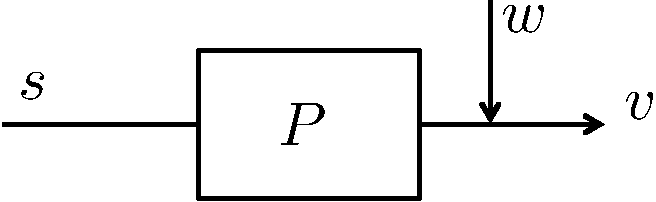
\includegraphics[width=.3\linewidth]{sys3.pdf}
\end{figure}

\begin{assumption}
  Assume that the measurement noise $w$ is Gaussian white with variance $\sigma_w^2$.
\end{assumption}

\begin{assumption}
  Assume that $P$ is FIR and the length of the impulse response is less than $T$. We parameterize
  the plant by its impulse response $p$.
\end{assumption}


\begin{definition}[Learning from open loop data]
  Learning from open loop data is to map the observation $(s,v)$ to a set of IQCs $\mc Q_P$.  The
  description of the unknown plant $P$ is in the form of a set of constraints on its input output
  signals.


  For example, under the assumptions, the observation $(s,v)$ gives the following constraint on the
  impulse response $p$ \rb{Doesn't this only hold in expectation/WHP? The constraint is fine, but it doesn't ``follow from the assumption''.}:
  \begin{align*}
    % &\; ( v_i - p*s_i) (v_i - p*s_i)^\top \preceq \sigma_w^2 I, \quad \tx{for }i= 1,\dots N. \\
    &\; \rb{||v_i - p*s_i||_2^2 \leq \sigma_w^2, \quad \tx{for }i= 1,\dots N. \tx{ (same thing)}}
  \end{align*}
  % Via the Schur complement, this is equivalent to
  % \begin{align*}
  % \bmat{\sigma_wI & v_i - T_ps_i \\ (v_i - T_ps_i)^T & \sigma_w} \succeq &\; 0\:,
  % \end{align*}
  % where $T_p$ is the (lower triangular) impulse response matrix of $p$.
  % \rb{Need to figure out how to efficiently write this as constraints on the inputs and outputs of $P$}

\end{definition}

\paragraph{Step 2,  collect closed  loop experiment data}
Run closed loop experiment with the candidate controller $K$ to obtain $M$ pairs of length-$T$ signals
$\{(r_i,y_i) : i=1,\dots, M\}$.
\begin{figure}[!ht]
  \centering
  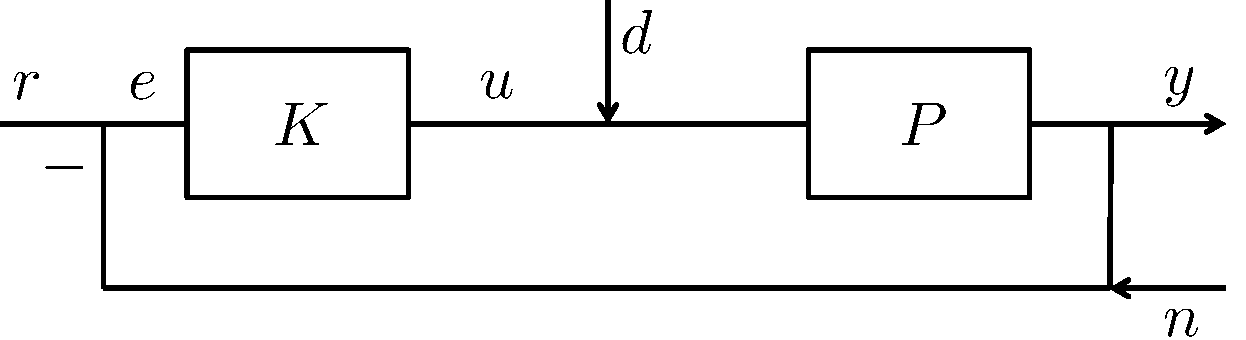
\includegraphics[width=.5\linewidth]{sys2.pdf}
\end{figure}

\begin{assumption}
  Assume that the disturbance $d$ and the measurement noise $n$ are Gaussian white with variance
  $\sigma_d^2$ and $\sigma_n^2$.
\end{assumption}


\paragraph{Step 3, controller invalidation}
Given the experiment data from Step 1 and Step 2, we want to check the if they are inconsistent with
the hypothesis that $K$ achieves the performance specification $T_{spec}$.
%
In particular, let $T_{\gamma}$ denote the achieved performance of the closed loop channel $d\to y$
and $n\to y$.

The invalidation of controller $K$ is to certify that there does not exist consistent noise signal
$(d_i, n_i)$ and impulse response of the plant $p$ such that:
\begin{align*}
  & (d_i,y_i), (n_i,y_i)\in T_{spec}, \quad\tx{(performance specification)}
  \\
  & y_i = p * ( k* (r_i-(y_i+n_i)) +d_i), \quad\tx{(constraint from $K$)}
  \\
  & \rb{||d_i||_2^2\leq \sigma_d^2 , \quad ||n_i||_2^2\leq \sigma_n^2, \quad \tx{for }i=
  1,\dots M,}
  \\
  & ||v_i - T_{s_i}p||_2^2 \leq \sigma_w^2, \quad \tx{for }i= 1,\dots N.
\end{align*}
where $T_{s_i}$ is the Toeplitz matrix generated by $s_i$.

By S-procedure, we can invalidate $K$ by solving an SDP feasibility problem, which provides
a sufficient condition for the invalidation.

\qq{Ross: make sure it is precise} \rb{I forget which covariance constraint things we came up with}
In the parlance of Smith and Dullerud, we have
\begin{align*}
P \triangleq &\; \bmat{-I & I & -I & K\\I & 0 & 0 & 0}\\
\Delta \triangleq &\; p \\
u \triangleq &\; r \\
w \triangleq &\; \bmat{d\\n}\\
W_{d,i}(w) = &\; \sigma_d^2 - ||d_i||_2^2\\
W_{n,i}(w) = &\; \sigma_n^2 - ||n_i||_2^2\\
W_{s,i}(w) = &\; \gamma_s^2||d_i||_2^2 - ||y_i||_2^2\\
W_{s^c,i}(w) = &\; \gamma_{s^c}^2||n_i||_2^2 - ||y_i||_2^2\\
\end{align*}
Instead of quadratic inequalities on $(z,v)$, we instead use quadratic inequalities on the plant impulse response vector $p$, which do not change the model invalidation setup.
\begin{align*}
Q_i(p) = &\; \sigma_w^2 - ||v_i - T_{s_i}p||_2^2 
\end{align*}
\rb{Todo: quadratic equality constraints}

\begin{remark}
  Note that the algorithm does not rely on the assumptions we made, but we need the assumptions to
  analyze the convergence and sample complexity.
\end{remark}

\begin{theorem}
  Let the general solution space of the linear equations
    \begin{align*}
      \bmat{-K & 0\\0&I}\bmat{r_i\\y_i} = &\; \bmat{I&-I&I&-I\\0&0&I&0}\bmat{d_i\\n_i\\v\\z}
    \end{align*}
  be given by \\
  \begin{align*}
    x(\xi) \triangleq&\; \bmat{d_1(\xi)\\\vdots\\d_M(\xi)\\n_1(\xi)\\\vdots\\n_M(\xi)\\v(\xi)\\z(\xi)}= x_0 + R\xi.
  \end{align*}

  Then, the model is invalidated if there nonnegative scalars $\tau_i,\ldots,\tau''''_i$ such that
  \begin{align*}
   W_0(\xi) + \sum_i \tau_i W_{d,i}(d_i(\xi)) + \sum_i \tau'_i W_{n,i}(n_i(\xi)) + \sum_i \tau''_i W_{s,i}(d_i(\xi)) + \sum_i \tau'''_i W_{s^c,i}(n_i(\xi)) + \sum_i \tau''''_i Q_i(p) \leq 0
  \end{align*}
  for all $(\xi,p)$.
\end{theorem}

\begin{corollary}
The model is invalidated iff there exist nonnegative scalars $\tau_i, \tau_i'$ such that
  \begin{align*}
  M_0 + \sum_i \tau_i\bmat{\tilde R^T A_i \tilde R &0 & A_i \tilde R\\0 & 0 & 0\\\tilde R^T A_i &0& \tilde x_0^TA_i\tilde x_0 + c_i} + \sum_j \tau_j'\bmat{0 & 0 & 0 \\ 0 & A_j' & b_j'^T\\0 & b_j' & c_j'} \preceq 0
  \end{align*}
\end{corollary}

where $x_0 = \bmat{\tilde x_0\\ x_{v,z}}$, $R = \bmat{\tilde R\\R_{v,z}}$, and $A_i,b_i,c_i,A'_j,b'_j,c'_j$ are given by...

\subsection{Sample complexity analysis}

Suppose the candidate controller $K$ can be invalidated for the true plant $P$.   Will
the algorithm consistently invalidate $K$ as $N,M\to\infty$.  How large $N$ and $M$ need to be so that the
algorithm can invalidate $K$ with high probability over the random noise in the experiments. How
does the sample complexity depends on the properties of $P$ and $K$?

Both open loop and closed loop data give us information about the unknown $P$, with which we try to
check the consistency.  We do explicit `learning' only with open loop data, while using the closed
loop data implicitly in the invalidation step.


\subsection{Experiment design}

Let the set of candidate $K$ be continuously parameterized. How to shrink the space efficiently to
obtain the set of unfalsified $K$.

% \paragraph{Naive questions}
% Why not replace Step 2 with IQC synthesis? why not replace Step 1 with point estimator plus
% uncertainty set? Advantage compared to existing 2-step ID and robust control?

\subsection{}
At some point, we might want include nuclear norm constraints which will restrict the complexity of the impulse response. To put nuclear norm contrains into our SDP framework, we can invoke the following lemma from [Maryam Fazels thesis]
\begin{lem} Let $X \in \mathbb{R}^{m \times n}$. Then, $\|X\|_* \le t$ if and only there exists matrices $Y \in \mathbb{R}^{m \times m}$ and $Z \in \mathbb{R}^{n\times n}$ for which
\begin{eqnarray}
\mathrm{Tr}(Y) + \mathrm{Tr}(Z) \le 2t & \text{and} \quad \begin{bmatrix} Y & X \\ X^T & Z \end{bmatrix} \succeq 0
\end{eqnarray}
\end{lem}


\end{document}

\newpage



\section{Controller invalidation for synthesis}
Robust synthesis is non-convex.  If we can do experiments to test different controllers, can we
``solve'' the synthesis problem by ruling out controllers which do not achieve the robust
performance? How to design the experiments to ``solve'' the synthesis problem in a more efficient
way?

%Decreases complexity by introducing uncertainty to the system and be more conservative.

\paragraph{To do list }
\begin{enumerate}
\item Find a simple parameterization of controller such that it works.
\item Sample complexity of invalidation?
\item Iterative id and invalidation?
\end{enumerate}



\paragraph{Setting}
Given:
\begin{itemize}
\item The part of plant that is known a priori, denoted by $P$.
\item Support of the of the unknown part of the plant $\Delta$: an {\em initial} description in the
  form of integral quadratic constraints on its input-output pair $(v,s)\in \mc Q_\Delta =
  \{Q_1,\dots, Q_L\}$.
  % (why not ssv or coprime factor)
\item Support of the controller $K$: a (discrete) set of candidate controllers $K \in \mc K =
  \{K_1,\dots, K_M\}$.
\item Support of the unobserved exogenous noise $w$: a bounded set in the form of IQCs $w\in \mc
  Q_{w}$.
\end{itemize}
Goal: find a controller $K\in\mc K$ that achieves robust stability and performance.

\paragraph{Basic idea}
The basic idea of ``controller invalidation experiments for synthesis'' is as follows.

Consider closed-loop system with a candidate controller $K\in\mc K$ in place.  Generate length $T$
observation $(u_t, y_t, z_t)_{t=1}^{T}$ generated by the closed loop system.

  Given $P, \mc Q_{\Delta}, \mc Q_{W}$, invalidate $K$ if there does not exist signal $(w_t, v_t,
  s_t)_{t=1}^{T}$ such that the following holds:
\begin{enumerate}
\item
  \begin{align*} (z,y,v) = P (u,w,s), \quad u = K z.
  \end{align*}
  Let $F_u(P,K)$ denote the linear fractional transformation, the two time domain equalities are
  equivalent to
  \begin{align*} (y,v) = F_u(P,K) (w,s).
  \end{align*}

\item IQCs for system  uncertainties are satisfied:
  \begin{align*} & w\in\mc Q_w, \quad (v,s) \in \mc Q_{\Delta}
  \end{align*}

\item Performance achieved.
  \begin{align*}
    (w,y) \in \mc Q_{T, \gamma}.
  \end{align*}
\end{enumerate}
\qq{convex?}

We need to do this test for every $K$ in the discrete set $\mc K$ to determine whether to keep it or
throw it out. If more than one $K$ is left, try:
\begin{itemize}
\item Get new observations for each $K$ with the same setup. Run the same invalidation procedure.
\item With the same observation, search for better performance so that sub-optimal controllers would
  be ruled out.
\end{itemize}



\begin{figure}[!ht]
  \centering
  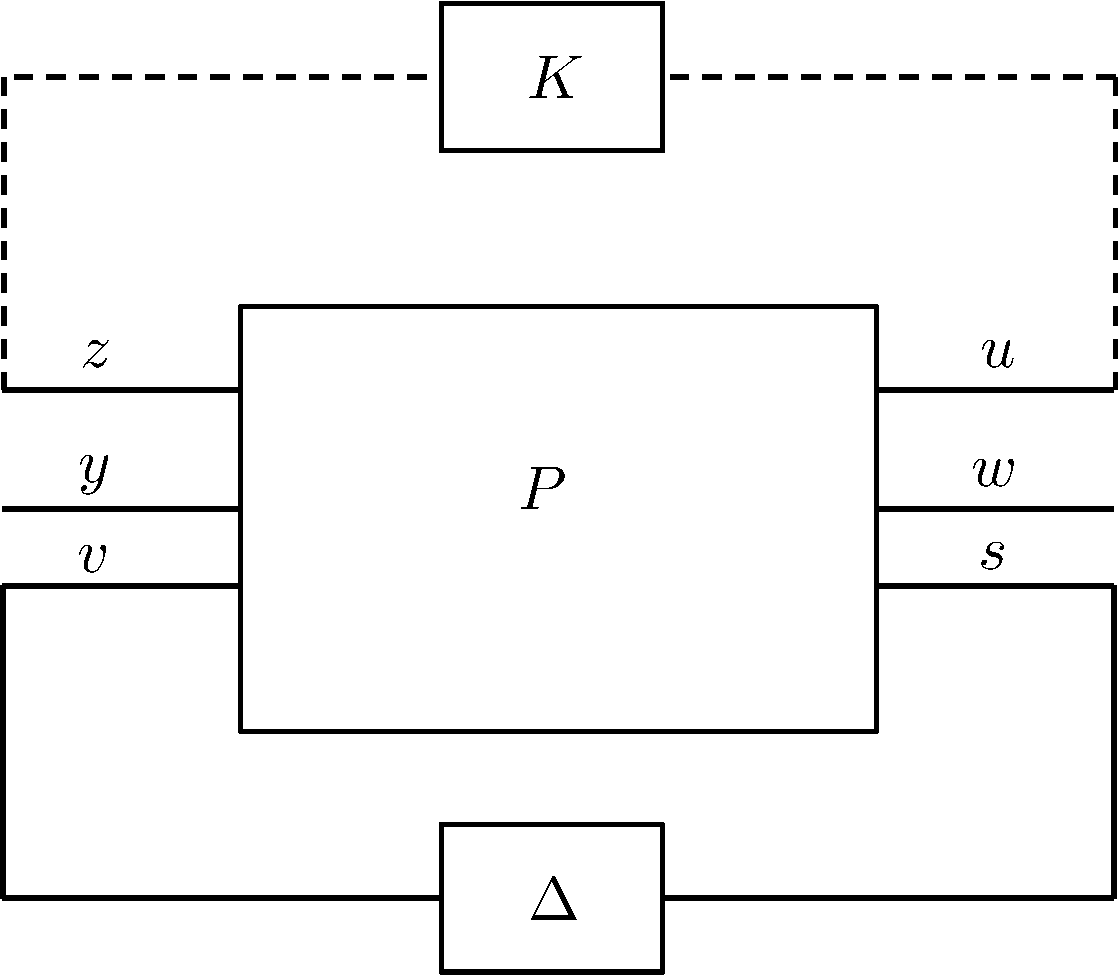
\includegraphics[width=.4\linewidth]{sys1.pdf}
\end{figure}




\paragraph{Discussions}
\begin{enumerate}
\item Start with a compact set for $\mc K$, we want to test one instance of $K$ and be able to rule
  out a measurable subset of $\mc K$.

  Experiment design. Note that in the closed loop id, choosing a particular controller $K$
  determines the $u$ input sequence. We want to select a controller $K\in \mc K$ so that we can
  shave of a large portion of $\mc K$ with the invalidation procedure.

\item Incorporate the information in the observed sequences to get a finer description of the
  uncertainty set $\Delta$, which would give us more invalidation power.

 For each $K_i\in\mc K$, we can potentially identify a set of $\Delta$ that are consistent with
  the observation for some $w\in\mc Q_{w}$. Denote it by $\Delta_{K_i}$.
  \\
  Find the tightest IQC description for the set $\cap_i \Delta_{K_i}$ and denote it by $\mc
  Q_{\Delta}'$.  Can we confidently rule out the subset of $\Delta$ in $\mc Q_{\Delta} \backslash
  \mc Q_{\Delta}'$?  No system in this subset can generate the observed sequences.








\bibliographystyle{plain}
\bibliography{invalid}

\end{document}
